\documentclass[a4paper]{article}
\usepackage[letterpaper, margin=1in]{geometry} % page format
\usepackage{listings} % this package is for including code
\usepackage{graphicx} % this package is for including figures
\usepackage{amsmath}  % this package is for math and matrices
\usepackage{amsfonts} % this package is for math fonts
\usepackage{tikz} % for drawings
\usepackage{hyperref} % for urls
\usepackage{pdfpages}

\title{Homework 1}
\author{Max Schemitsch}
\date{2/13/2019}

\begin{document}
\lstset{language=Python}

\maketitle

\section{Problem 1.4}

\subsection{A) and B)}
Using the code found in 'Master PLA.py', we can generate a linearly separable data set of size 20 with target function $f$ and final hypothesis $g$.

\begin{figure}[h]
  \begin{center}
    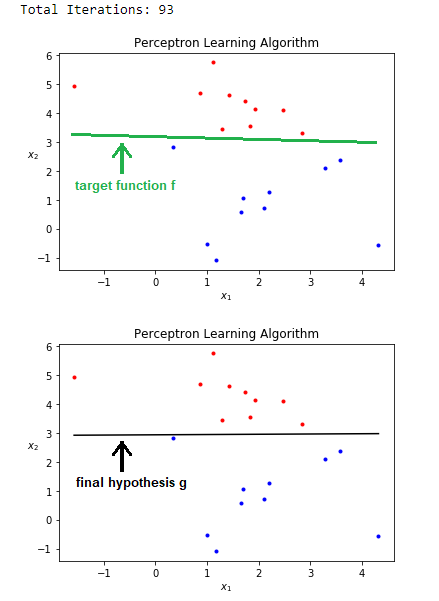
\includegraphics[width=80mm,scale=0.8]{problem14AB.png}
  \end{center}
\end{figure}

After 93 iterations, we can see that $f$ is very close to $g$. They both satisfy the division of classes.

\newpage

\subsection{C)}
We can do the same thing as before with another random data set.

\begin{figure}[h]
  \begin{center}
    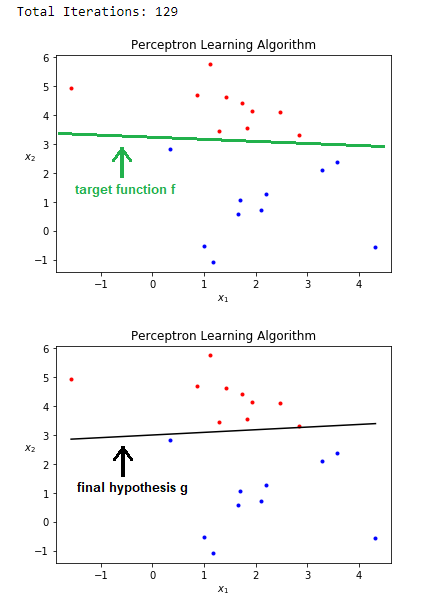
\includegraphics[width=80mm,scale=0.8]{problem14C.png}
  \end{center}
\end{figure}

After 129 iterations, this particular $f$ function is close to this particular $g$ function. My initial target function, however, had a negative slope as opposed to the positive slope of $g$.

\newpage

\subsection{D)}
We obtain similar results with a size of 100. We have 8 iterations and a similar $f$ and $g$.

\begin{figure}[h]
  \begin{center}
    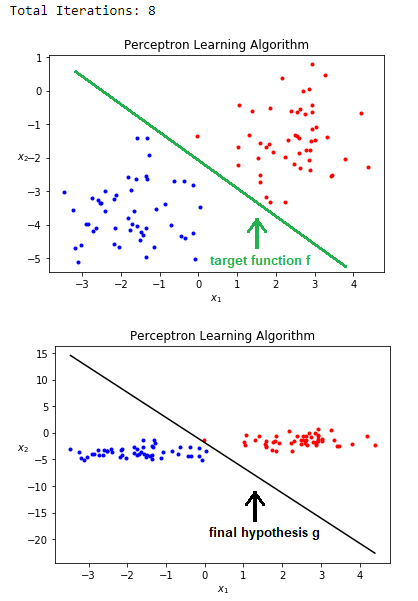
\includegraphics[width=80mm,scale=0.8]{problem14D.png}
  \end{center}
\end{figure}

\newpage

\subsection{E)}
We obtain another set of similar results with a size of 1000.

\begin{figure}[h]
  \begin{center}
    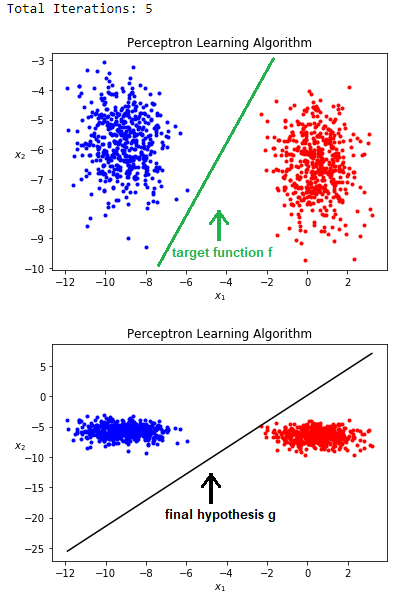
\includegraphics[width=80mm,scale=0.8]{problem14E.png}
  \end{center}
\end{figure}
We can see that while my $f$ function is roughly in the middle of the data sets, $g$ sits right on the border of the red classified data.

\newpage

\subsection{F)}
In order to modify the number of dimension from 2 to 10, we must alter part of the code found in 'Master PLA.py'. We must set $n features=10$ and make sure we have $np.zeros(11)$. We can then run the code to obtain this:

\begin{figure}[h]
  \begin{center}
    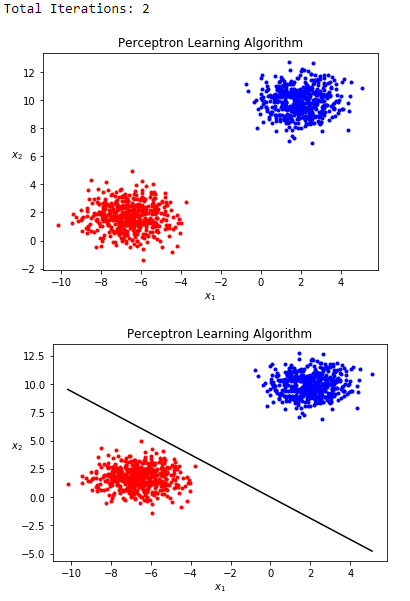
\includegraphics[width=80mm,scale=0.8]{problem14F.png}
  \end{center}
\end{figure}

This particular random data set only took two iterations to converge.

\newpage

\subsection{G)}
In order to run the experiment 100 times and collect 100 different iteration counts, we apply this bit of code before and after our $main()$:
\begin{lstlisting}[frame=single]
itlst = []
    for x in range(100):
......
itlst.append(it)
    print(itlst)
\end{lstlisting}

With our list of iteration counts, we can then plot a histogram using this bit of code:
\begin{lstlisting}[frame=single]
his = plt.hist(itlst, bins = [0, 1, 2, 3, 4, 5, 6, 7]);
fig, ax = plt.subplots()
offset = 0
plt.bar(his[1][1:], his[0])
ax.set_xticks(his[1][1:] + offset)
ax.set_xticklabels( ('0', '1', '2', '3', '4', '5', '6', '7') )
plt.xlabel("Number of Iterations")
plt.ylabel("# of Iterations Count")
\end{lstlisting}
This code produces our histogram:
\begin{figure}[h]
  \begin{center}
    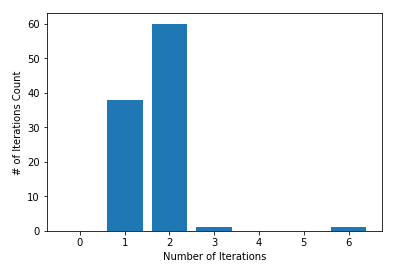
\includegraphics[width=80mm,scale=0.8]{problem14G.png}
  \end{center}
\end{figure}

We can see that the majority (around 60) of experiments took 2 iterations and roughly 38 of them took only 1 iteration. Only one experiment needed 3 iterations and another needed 6.
\subsection{H)}
When working through this homework, it seemed the that most important aspect of this PLA was the data set size. I could not get a 1000 size data set to run the algorithm when I had the random state set equal to a value. It would never get to the point of converging, and run forever. When I removed the random state variable, the algorithm worked almost every time. It also seems that the running time for this PLA was linked directly to the data set size (if felt exponentially longer from 20 then to 100 and finally to 1000). Dimension size also directly increased the running time as well.

\end{document}